

\documentclass[a4paper,12pt]{article}

\usepackage{amsmath}
\usepackage{amsfonts}
\usepackage{amssymb}
\usepackage{amsthm}
\usepackage{amsrefs}
\usepackage[english]{babel}
\usepackage[all]{xy}
\usepackage{graphics,color}
\usepackage{ textcomp }
\usepackage{graphicx}
\usepackage{pdfpages} 

\setlength{\parindent}{0cm}
\setlength{\parskip}{0.5\baselineskip}


\newcommand{\HRule}{\rule{\linewidth}{0.5mm}}


\begin{document}

\begin{titlepage}

\begin{center}


\HRule \\[0.4cm]
{ \huge \bfseries Discussieforum}\\[0.4cm]
\HRule \\[0.4cm]

\vfill

\end{center}

\begin{minipage}{0.4\textwidth}
\begin{flushleft} \large
\emph{Gemaakt door:}\\
Michael Chen\\ Jenniger Roeting\\ Kyllian Broers \\ Max Bevelander \\
\emph{Groep: Webdb13KIC1}
\end{flushleft}

\end{minipage}
\vfill
{\large \today}

\end{titlepage}

\newpage
\begin{center}
{ \LARGE \bfseries Inhoudsopgave}
\HRule \\[0.5cm]
\end{center}
\tableofcontents

\newpage
\begin{center}
\part[Informatie voor de klant]{ Informatie voor de klant}
\HRule \\[0.5cm]
\end{center}

\begin{center}
\section[Inleiding]{Inleiding}
\HRule \\[0.5cm]
\end{center}
De opdracht is het bouwen van een discussieforum voor een bedrijf, waardoor gebruikers eenvoudiger met elkaar contact kunnen houden. Zo kunnen klanten bijvoorbeeld vragen stellen over de producten van het bedrijf of feedback geven op het bedrijf of de producten. Er moet een hi\"erarchische structuur in het forum zitten, zodat niet alle gebruikers dezelfde rechten hebben.
Voor dit forum zullen er drie soorten gebruikers zijn: beheerders, ingeschreven gebruikers en mensen die niet ingeschreven staan in het forum.\\

Beheerders\\
De mensen van het bedrijf zelf zijn  de beheerders van het forum. Zij moeten nieuwe categorieën kunnen maken en verwijderen. Het moet mogelijk zijn om per forum te kiezen of de ingezonden berichten direct in het forum geplaatst worden of eerst gescreend moeten worden door de beheerders.\\

Gebruikers\\
De gebruikers zijn klanten die zich voor  het forum geregistreerd hebben. Zij kunnen onder andere de goedgekeurde berichten lezen, zelf berichten plaatsen en reageren op andere berichten. \\

Niet-gebruikers\\
De niet-gebruikers kunnen alleen goedgekeurde berichten lezen. Het forum is voor de niet-gebruikers erg gelimiteerd. Om gebruiker te worden, kunnen zij zich registeren op het forum. \\


\begin{center}
\section[Functionele eisen]{Functionele Eisen}
\HRule \\[0.5cm]
\end{center}
Een discussieforum bestaat uit de volgende basis aspecten:
\begin{itemize}
\item Homepagina
\item Registratiepagina
\item Inlogpagina
\item Forum
\item Ledenlijst
\item Profielpagina
\item FAQ-pagina
\item Administrator paaneel
\end{itemize}

Om dit zo duidelijk mogelijk weer te geven is het van belang dat het forum een aantrekkelijk uiterlijk heeft dat past bij het bedrijf. Daarnaast moet een nieuwe gebruiker, direct zijn of haar weg kunnen vinden op het forum. Het is dus van belang dat het forum overzichtelijk is en dat er makkelijk te navigeren is door de pagina's. Gebruikersvriendelijkheid wordt versterkt door het toedelen van administrator rollen. Dit zijn aangwezen gebruikers die de orde op het forum handhaven. Daarnaast is een veilige omgeving essenti\"eel. Daarom zal er gezorgd worden dat opslag en uitwisseling van gebruikersgegevens zo veilig mogelijk plaats zal vinden.


\begin{center}
\section[Ontwerp Beslissingen]{Ontwerp Beslissingen}
\HRule \\[0.5cm]
\end{center}
\subsection[Homepagina]{Homepagina}
De homepagina bestaat uit een korte introductie over de inhoud van de website. Daarnaast worden op de homepagina de 10 meest recente en de 10 meest populaire berichten weergegeven. Hierdoor kan de gebruiker in \'e\'en oogopslag zien, welke onderwerpen nieuw zijn en uit welke onderwerpen de bezoeker mogelijk de meeste informatie kan halen. Een onderwerp is populair zodra het meer dan 15 reacties heeft. De onderwerpen die in deze lijsten verschijnen zijn klikbare links die verwijzen naar het berichtenoverzicht van het desbetreffende ondwerp.\\



\subsection[Registratiepagina]{Registratiepagina}
De registratiepagina wordt geladen in de index pagina, daarna wordt als er ingelogd is doorverwezen naar de homepagina. als er niet ingelogd is wordt er gekeken of het registratieformulier gesubmit is, is dit niet het geval dan wordt het registratieformulier geladen, in dit formulier wordt van de gebruiker gevraagd een aantal verplichte en niet verplichte velde in te vullen, de verplichte velden zijn aangegeven door een asterix om dit te verduidelijken en als die niet ingevuld zijn wordt daar ook een melding voor gegeven nadat het formulier gesubmit is. De velden zonder asterix zijn optioneel en het is dan ook geen probleem als de gebruiker hier niks invult. Het formulier is geordend in een tabel om een duidelijke representatie te geven aan de gevraagde gegevens, er zijn 2 kolommen waarbij in de linker staat wat de gevraagde invoer is en in de rechterkolom het daarbij behorende veld. Zo kan de gebruiker op een comfortabele manier het formulier invullen. Onder de tabel staat een registreerknop waarmee de gebruiker zijn gegevens laat registreren in de database. \\
Het formulier verwijst eerst naar zichzelf waarbij alle gegevens worden gecheckt op een correcte invoer en beveiligd tegen injectie. Zodra dit bij een veld het geval is zal er een error achter dit veld komen te staan om de gebruiker aan te duiden dat het veld incorrect is ingevuld. De overige ingevulde gegevens die wel door de check heen zijn gekomen blijven daarbij gewoon is de velden staan zodat het gehele formulier niet in zijn geheel opnieuw hoeft te worden ingevoerd. Als uiteindelijk alle gegevens door de checks heen zijn gekomen wordt een pagina laten zien waar aangegeven wordt dat het registreren in gelukt en dat een mail naar de gebruiker is gestuurd.\\
 Deze mail dient al verwelkoming en verificatie van het account van de gebruiker, dit voorkomt het nodeloos aanmaken van accounts. In de mail staan twee links, een om het account te verifiëren en een ander om aan te geven dat de mail niet voor de ontvangen persoon was bedoelt zodat als een persoon niet met het email adres van een vreemde kan registreren. Na de verificatie via de link in de mail is de gebruiker volledig geverifieerd.\\
Een paar opmerking voor de gegevens die de gebruiker ingevoerd heeft in het formulier:
\begin{itemize}
\item Een gebruiker moet een unieke gebruikersnaam invoeren, over de gehele site en in de database word zo gebruik maakt van de gebruikersnaam dat elke gebruiker een unieke gebruikersnaam moet hebben, bovien is deze naam ook de naam waarmee de gebruiker zicht representeert op de site en zodoende is een unieke gebruikersnaam een stuk duidelijker voor iederee.
\item Ook het e-mailadres van de gebruiker moet uniek zijn zodat er geen meerdere account gekoppeld kunnen worden aan hetzelfde emailadres 
\item De avatar die de gebruiker optioneel kan invoeren wordt opgeslagen in de map avatars op de server van de site. De rechte voor deze map zijn zo dat ook anderen erin kunnen schrijven. Dit is nodig om de avatar te kunnen uploaden naar de server. Wij hebben andere methodes bedacht zoals bijvoorbeeld ‘scp’. Dit werkte in principe wel maar omdat daar een gebruikersnaam en wachtwoord van een van de mensen het team voor nodig hebben wij dit niet gedaan. Dit omdat er nu gewerkt wordt op een server waar vele anderen ook toegang tot hadden, wat bij een eigen server voor de site niet het geval zou zijn en wij de middelen en tijd niet hebben om het zodanig via scp te doen dat die gegevens afgeschermd zouden zijn.
\end{itemize}

Ter conclusie zijn bij de verdere gegevens die ingevuld worden de hoogste veiligheidsmaatregelen genomen om zowel de server , de database als de gebruiker te beschermen. Dit door middel van versleutelingen en checks om de invoer te controleren.

\subsection[Inlogpagina]{Inlogpagina}
Voor de inlog pagina is er gekozen voor een link die weliswaar niet in de menubalk zit, maar toch vanuit elke pagina te bereiken is. Deze zit in de rechterbovenhoek van de pagina, boven de menubalk. We hebben hiervoor gekozen omdat de inlog pagina niet een direct onderdeel vormt van de inhoud van het forum.
Op de inlog pagina wordt gevraagd om de invoer van twee gegevens, namelijk het wachtwoord en de gebruikersnaam van de gebruiker. Daarnaast zijn er twee links onder het inlogformulier, een link waarbij een nieuw wachtwoord opgevraagd kan worden en een link om te registreren indien de gebruiker nog geen account heeft. Deze links verhogen het gebruikersgemak.
Afsluitend, als alles ingevuld is, kan er op de "Sign in" button gedrukt worden. Indien er een fout is gemaakt, dan zal dit gemeld worden en kan de gebruiker een nieuwe inlogpoging doen. Zodra het inloggen geslaagd is, is de gebruiker ingelogd en kan deze gebruik maken van de vele functies op het forum.\\


\subsection[Forum]{Forum}
De indeling van het forum is zodanig, dat het overzichtelijk is en intuitief in gebruik. Ook zonder handleiding moet een gebruiker in staat zijn om berichten te kunnen plaatsen en onderwerpen te kunnen vinden.
Het forum bestaat uit drie onderdelen. Een overzicht met de categorie\"en, een overzicht van de onderwerpen binnen een zekere categorie en een overzicht van de berichten in een zeker onderwerp. In het overzicht met categorie\"en worden categorie\"en weergegeven waarin de gebruiker onderwerpen kan plaatsen. Het indelen in categorie\"en maakt het forum overzichtelijk voor de gebruiker. De gebruiker kan zo zien waar deze moet zijn om een antwoord op zijn of haar vraag te vinden. Het overzicht met categorie\"en bestaat uit klikbare links, waarna de gebruiker terechtkomt in het onderwerpenoverzicht. Dit overzicht bestaat uit een lijst met alle onderwerpen die geplaatst zijn in een zekere categorie. Deze lijst bestaat uit klikbare links naar het berichtenoverzicht van een zeker onderwerp. Wanneer de gebruiker ingelogd is, heeft deze de mogelijkheid om een nieuw onderwerp te plaatsen door op de daarvoor bestemde knop te drukken. Voordat dit onderwerp zal verschijnen in het onderwerpenoverzicht, dient deze eerst goedgekeurd te worden door een administrator, zodat spamberichten of berichten in een verkeerde categorie voorkomen worden. Het berichtenoverzicht van een zeker onderwerp bestaat uit het beginbericht, waarmee het onderwerp geopend is en alle reacties van andere gebruikers. Indien een gebruiker ingelogd is, heeft deze de mogelijkheid om een reactie te plaatsen door zijn of haar reactie te schrijven, onderaan de pagina. Daarnaast heeft de gebruiker de mogelijkheid om de inhoud van zijn of haar eigen berichten te verwijderen en berichten van anderen als spam te rapporteren.\\


\subsection[Ledenlijst]{Ledenlijst}
Het forum is niet compleet zonder een ledenlijst. Hierin worden alle mensen die zich geregistreerd hebben als gebruiker weergegeven. Mensen die niet geregistreerd staan, kunnen de ledenlijst niet zien. Als een niet-gebruiker op de ledenlijst klikt, wordt diegene direct doorverwezen naar de inlogpagina. Het enkel weergeven van de gebruikersnamen in de lijst was naar onze mening niet aantrekkelijk, dus hebben we besloten ook nog de registratiedatum, het aantal berichten die de gebruiker heeft geplaatst, het e-mail adres van de gebruiker en het account-type van de gebruiker weer te geven. Als extra functie zijn de gebruikersnamen klikbare links. Als op een naam wordt klikt, wordt er doorverwezen naar zijn of haar profiel. \\

 
\subsection[Profiel]{Profiel}
Ieder lid van het forum heeft een eigen profiel pagina ter beschikking, die de gebruiker kan bewerken, om zo zijn of haar account persoonlijker te maken. Zo kan de avatar afbeelding en de quote veranderd worden en kan de gebruiker een leeftijd, een land en een persoonlijke tekst toevoegen. Ook is er de mogelijkheid om het wachtwoord te veranderen. Dit is vooral handig wanneer de gebruiker zijn of haar wachtwoord is vergeten en een nieuw, automatisch gegenereerd, wachtwoord heeft ontvangen. Dit zijn vaak onhandige wachtwoorden, waarvan het handig is om deze te wijzigen. Indien een gebruiker ook een administrator van het forum is, beschikt diegene ook een "adminitrator panel" in zijn of haar profiel. \\


\subsection[Administrator Paneel]{Administrator Panel}
Om het berichtenverkeer in het forum te handhaven, zijn er administrators toegewezen. De administrators kunnen enkel bepaald worden door de website beheerders. Administrators hebben hun eigen panel, deze is toegankelijk via hun eigen profiel. Hier vinden zij een overzicht van de andere administrators op het forum, een lijst met nog goed te keuren onderwerpen, een lijst met spamrapportages en een overzicht van nog niet geactiveerde accounts. Daarnaast hebben administrators de mogelijkheid om gebruikersaccounts te blokkeren wanneer zij voor overlast op het forum zorgen. De taken van een administrator zijn het blokkeren van gebruikers die de rust op het forum verstoren, het goed- of afkeuren van nieuwe onderwerpen, het nakijken van spamrapportages en het eventueel verwijderen van deze berichten, het verwijderen van onredelijke berichten en het verwijderen van gebruikersaccounts die nog niet geactiveerd zijn en langer dan twee weken terug aangemaakt zijn. \\


\subsection[FAQ Pagina]{FAQ Pagina}
Om de niet-gebruikers en nieuwe gebruikers van het forum een handje te helpen, is er ook een FAQ-pagina aanwezig. Deze pagina is voor iedereen toegangkelijk. Daarin staan alle meest gestelde vragen met de bijbehorende antwoorden. De vragen zijn weergegeven als links en de antwoorden van die vragen komen te voorschijnen als er op geklikt wordt. Dus als gebruikers vragen hebben of problemen ondervinden, kunnen zij eerst de FAQ-pagina raadplegen. Om het forum netjes te houden, staan er ook een aantal regels vermeld in de FAQ-pagina waar de gebruikers zich aan dienen te houden.



\begin{center}
\section[Handleiding]{Handleiding}
\HRule \\[0.5cm]
\end{center}
Ten eerste zullen de functies worden besproken waarover een niet ingelogde gebruiker beschikt. Vervolgens zal een handleiding volgen voor het registreren en inloggen. Tenslotte zullen de functies voor een ingelogde gebruiker besproken worden.\\
De gebruiker komt als eerste op de home pagina, waar de 10 meest recente onderwerpen en de tien meest populaire onderwerpen weergegeven worden. Ieder onderwerp bevat een link naar de pagina van het desbetreffende onderwerp met desbetreffende tekst en reacties.
Door in de menubalk op "forum" te klikken wordt te gebruiker verwezen naar het forum. Deze knop is op iedere pagina van de website aanwezig. Hier zal een overzicht gevonden worden met alle categorie\"en.  Achter de categorie staat ook het aantal onderwerpen in de desbetreffende categorie. Door op een categorie te klikken wordt de gebruiker verwezen naar het overzicht van alle onderwerpen die behoren tot die categorie. De onderwerpen zijn geordend op datum dat ze zijn aangemaakt. Per pagina worden er twintig onderwerpen weergegeven. Onderaan de pagina kan door de pagina's gebladerd worden. Bij ieder onderwerp staat wanneer de laatste reactie is geplaatst in dat onderwerp. Door op een onderwerp te klikken komt de gebruiker op het overzicht van de berichten binnen een onderwerp. Voor ieder bericht is te zien van welke gebruiker de reactie is, inclusief een link naar het profiel van deze gebruiker, wanneer het bericht geplaatst is, het bericht zelf, een eventuele quote en of de gebruiker een administrator is of een gewone gebruiker. Het laatste wat een niet ingelogde gebruiker kan doen, is het bezoeken van de FAQ pagina, waar de tien meestgestelde vragen staan. Door te klikken op een vraag wordt de gebruiker doorgestuurd naar het antwoord. De "Go Back" link die aanwezig is op deze pagina, verwijst de gebruiker terug naar de FAQ-pagina.\\
Nu zal een handleiding volgen voor het registreren en inloggen. De gebruiker kan zich registreren door op "Register" te klikken, rechtsboven. De velden met een ster zijn verplichte velden. De velden zonder ster hoeven niet ingevuld te worden. Men kan een avatar uploaden. Dit is een afbeelding die weergegeven wordt bij de reacties van de gebruiker en op de profielpagina van de gebruiker. Als men eenmaal geregistreerd is, is het proces bijna klaar. Er zal een e-mail gestuurd worden naar het ingevulde e-mail adres. In deze e-mail staat een link, waarmee het account geverifi\"eerd kan worden. Hierna kan de gebruiker inloggen. \\
Eenmaal ingelogd is er een scala aan mogelijkheden waarover de gebruiker beschikt. De gebruiker kan naar de ledenlijst gaan wanneer deze op "Members" klikt in de menubalk. Rechtsboven kan de gebruiker op zijn of haar eigen gebruikersnaam klikken. De gebruiker wordt doorverwezen naar zijn of haar eigen gebruikersprofiel. Het profiel kan aangepast worden door op "edit profile" te klikken. Ook kan het wachtvoord van de gebruiker aangepast worden door op "change password" te klikken. Rechtsboven is ook een knop "Log out" te vinden, om uit te loggen. Het belangrijkste is natuurlijk het forum. Als de gebruiker ingelogd is, kunnen er nieuwe berichten gestart worden of gereageerd worden op al bestaande onderwerpen. Zoals ook niet-ingelogde gebruikers kan er geklikt worden het onderwerp waarop me wilt reageren. Bovenin staat nu een knop met “New subject”. Als hierop geklikt wordt kan de gebruiker een nieuw onderwerp plaatsen. Hier kan de gebruiker het onderwerp kiezen, de categorie waarin het onderwerp toebehoort en de vraag of het bericht dat de gebruiker wilt plaatsen. Voordat het onderwerp verschijnt in de lijst met onderwerpen, zal het onderwerp eerst gecheckt worden door administrators op ongewenste inhoud, waarna het, als het is goedgekeurd, wordt geplaatst in de gekozen categorie. Als het onderwerp eenmaal in het forum staat naar beneden gescrolld worden, net zoals bij elk ander onderwerp, om daar een nieuwe reactie schrijven.


\begin{center}
\section[Reflectie]{Reflectie}
\HRule \\[0.5cm]
\end{center}
{\bfseries Doelen die bereikt zijn:}\\
\begin{itemize}
\item Registreerpagina: 
Je moet als gebruiker kunnen registreren om het forum te kunnen gebruiken.
\item Inlogpagina:
Er moet een inlogpagina aanwezig zijn, zodat mensen als gebruikers kunnen inloggen.
\item Het forum met de geplaatste berichten:
De gebruikers moeten op het forum berichten kunnen plaatsen en op bestaande berichten reageren.
\item Home pagina:
De 10 meest recente berichten en 10 meest populaire berichten worden in de home pagina weergegeven.
\item Profielpagina:
Ieder lid heeft een eigen profiel.
\end{itemize}

Extra aspecten die toegevoegd zijn aan het forum:
\begin{itemize}
\item Op de inlogpagina staat een extra link “password forgotten”. Als een gebruiker zijn of haar wachtwoord is vergeten, dan wordt er via de mail een nieuw wachtwoord verstuurd naar de gebruiker;
\item Op het forum is een ledenlijst aanwezig;
\item Regels die gebruikers op het forum moeten naleven en meest gestelde vragen in de FAQ-pagina;
\item Knopje om ongepaste berichten te melden;
\item Administratorpanel: wordt weergeven op profielpagina als diegene een administrator is;
\item Een gebruiker kan indien gewenst zijn of haar wachtwoord wijzigen.
\end{itemize}
{\bfseries Doelen die niet bereikt zijn:}
\begin{itemize}
\item Zoekmachine;
\item Javascript gebruiken om velden te controleren waar gebruikers gegevens moeten invullen bijvoorbeeld bij het registreren, inloggen en het wijzigen van het profiel;
\item Personal Message-systeem voor de leden;
\item Status van de leden: online of offline op het forum;
\end{itemize}

De bovenstaande doelen zijn niet bereikt en dat komt vooral wegens gebrek aan tijd.


\newpage
\begin{center}
\part[Informatie voor ICT]{Informatie voor ICT}
\HRule \\[0.5cm]
\end{center}


\begin{center}
\section[Software]{Software}
\HRule \\[0.5cm]
\end{center}
De programmeeromgeving dient te bestaan uit een editor voor PHP en HTML, het programma dat hiervoor gebruikt kan worden is afhankelijk van de voorkeur van de beheerder. Relatief eenvoudige editors zoals Gedit zijn voldoende, maar ook kunnen programma's als Dreamweaver en Eclipse gebruikt worden. Daarnaast is er een SFTP of SSH file transfer benodigd. Hiervoor is WinSCP aanbevolen. De server moet voorzien zijn van LAMP software.


\begin{center}
\section[Installatieprocedure]{Installatieprocedure}
\HRule \\[0.5cm]
\end{center}
Voor het gebruik van dit forum op een eigen server is een kort installatie proces van toepassing, hieronder staat aangegeven welke stappen nodig zijn en een uitleg daarbij.\\
Voor het uitvoeren van deze website moet de server voorzien zijn van standaard LAMP software.\\

Het installeren benodigd de volgende stappen
\begin{itemize}
\item Creeer een map public\_html, in deze map zullen alle bestanden voor de site komen te staan.
\item Pak codes.zip uit en kopieer de bestanden uit de map codes naar de map public\_html, dit zijn alle pagina’s en php code voor de site.
\item Kopieer de map images naar public\_html, hierin staan de alle plaatjes die op de site gebruikt worden.
\item Kopieer de map avatars naar public\_html, de rechten voor deze map moeten rwxr-xr-x  zijn. In deze map staat het bestand avatars.png, dit is het standaard plaatje dat als avatar wordt gebruikt, verder zal deze map zich vullen met de avatars die gebruikers voor zichzelf uploaden.
\item Ga naar het bestand db\_con.php, dit bestand zet een connectie op met de database, verander de 2 parameter van de PDO functie naar uw databasenaam, de derde parameter naar uw database gebruikersnaam en de vierde parameter naar uw database wachtwoord.
\item Ga naar de database waarvoor u hierboven de gegevens heeft genoteerd en importeer webdb13KIC1.sql. nu staan de tabellen voor de site in uw database.
\item De site is nu volledig geïnstalleerd en werkzaam, als u gebruikers een administrator status wilt geven zet dan in de kolom account\_type de waarde van ‘usr’ naar ‘adm’.
\end{itemize}

\begin{center}
\section[Structuur]{Structuur}
\HRule \\[0.5cm]
\end{center}
Bijna alle pagina’s maken gebruik van de connectie met de database. Alleen de FAQ-pagina maakt geen gebruik ervan. Er wordt een connectie gemaakt met de database door het bestand 'db\_con.php'. In die database staan drie tabellen beschreven: 
\begin{itemize}
\item user\_data: alle gegevens van de geregistreerde gebruikers;
\item subjects: alle berichten die geplaatst zijn door de gebruikers van het forum;
\item posts: alle reacties van gebruikers op die berichten.
\end{itemize}

\subsection[Registratie]{Registratie}
Het registeren gebeurt in het 'registerform.php' bestand. Daar worden de ingevulde velden (gegevens van de gebruiker) in de tabel 'user\_data' geplaatst. Natuurlijk worden de ingevulde velden eerst gecontroleerd. Na het invoeren van de gegevens wordt “register.php” aangeroepen. Daarin worden de velden gecontroleerd. Zo mag bijvoorbeeld een “username” geen spaties bevatten en het moet uniek zijn. Op deze manier worden alle velden gecontroleerd. 

\subsection[Inloggen]{Inloggen}
Tijdens het registeren zijn de velden, als alles goed is verlopen, opgeslagen in de tabel 'user\_data'. Om te kunnen inloggen, moet de gebruiker zijn of haar gebruikersnaam en wachtwoord invullen dat beschreven is door het bestand 'inlog.php'. Na het invoeren wordt de 'checklogin.php' aangeroepen. Daar wordt gekeken of de gebruikersnaam en het wachtwoord in de database staan en of het bij die gebruiker overeenkomen. Als alle stappen zijn verlopen zonder fouten, dan is de gebruiker ingelogd.

\subsection[Ledenlijst]{Ledenlijst}
De gebruikers die zich op het forum hebben geregistreerd en hun account hebben geactiveerd komen in de database te staan. Met behulp van de een query worden de gegevens per gebruiker opgehaald uit de database en vervolgens wordt daar een mooi lijst van gemaakt. 

\subsection[Profiel]{Profiel}
De gegevens van de gebruiker worden getoond in het profiel. Indien gewenst kan het profiel en het wachtwoord van de gebruiker bewerkt worden en kunnen er zo nieuwe gegevens aan de database worden toegevoegd. Het 'editprofile.php' bestand is het formulier om de nieuwe gegevens in te vullen. Vervolgens worden deze velden gecontroleerd door het bestand 'profiel.php'. Voor het wachtwoord is er een apart bestand genaamd 'changepasswordform.php'. Eveneens wordt het invoer gecontroleerd door het bestand 'changepassword.php'. 

\subsection[Forum]{Forum}
Als een gebruiker een eigen bericht maakt of op andere berichten reageert, wordt dat opgeslagen in de tabellen subjects en posts. Met behulp van queries worden de berichten met de bijbehorende reacties getoond. Ook hier wordt al het invoer gecontroleerd voordat ze in de database worden ingevoerd.\\


\begin{center}
\section[Instructies]{Instructies}
\HRule \\[0.5cm]
\end{center}
Voor het onderhouden van de website zijn een aantal dingen van belang. Als eerste is het van belang om ervoor te zorgen dat er voldoende administratoren aangewezen worden en om de activiteit van deze in de gaten te houden. Het is namelijk van belang dat er adequaat gereageerd kan worden op de activiteit in het forum. Voor gebruikers is het onprettig als het lang duurt wanneer berichten goedgekeurd worden en wanneer er lastige gebruikers zijn op het forum.\\
Daarnaast is het van belang dat de database onderhouden wordt. Onderwerpen die verwijderd worden van de website, worden niet daadwerkelijk verwijderd uit het forum. Dit is gedaan, zodat fouten nog hersteld kunnen worden. Echter, onderwerpen die lang geïnactiveerd worden, kunnen het beste uit de database verwijderd worden, om deze van onnodige data te ontdoen.\\
Ook is het van belang dat de werking van de website in de gaten wordt gehouden. De website moet in alle browsers goed kunnen werken, ook na updates. Het is van belang om dit te blijven controleren en de code zonodig aan te passen. \\
Tenslotte zijn wij van mening dat er ten alle tijde gestreefd moet worden naar een optimale gebruikersvriendelijkheid en veiligheid. Zoals reeds besproken zijn er onder de tijdsdruk bepaalde keuzes hierin gemaakt. Dit neemt echter niet weg dat het eindproduct definitief moet blijven. Wanneer het website beheer ondervindt dat bepaalde onderdelen beter beveiligd kunnen worden, of bepaalde toevoegingen het gebruikersgemak kunnen vergroten, dan zullen wij dit enkel stimuleren.


\begin{center}
\section[Datamodel]{Datamodel}
\HRule \\[0.5cm]
\end{center}

De gehanteerde structuur voor de webpagina's en de database zijn op de volgende pagina's te zien.
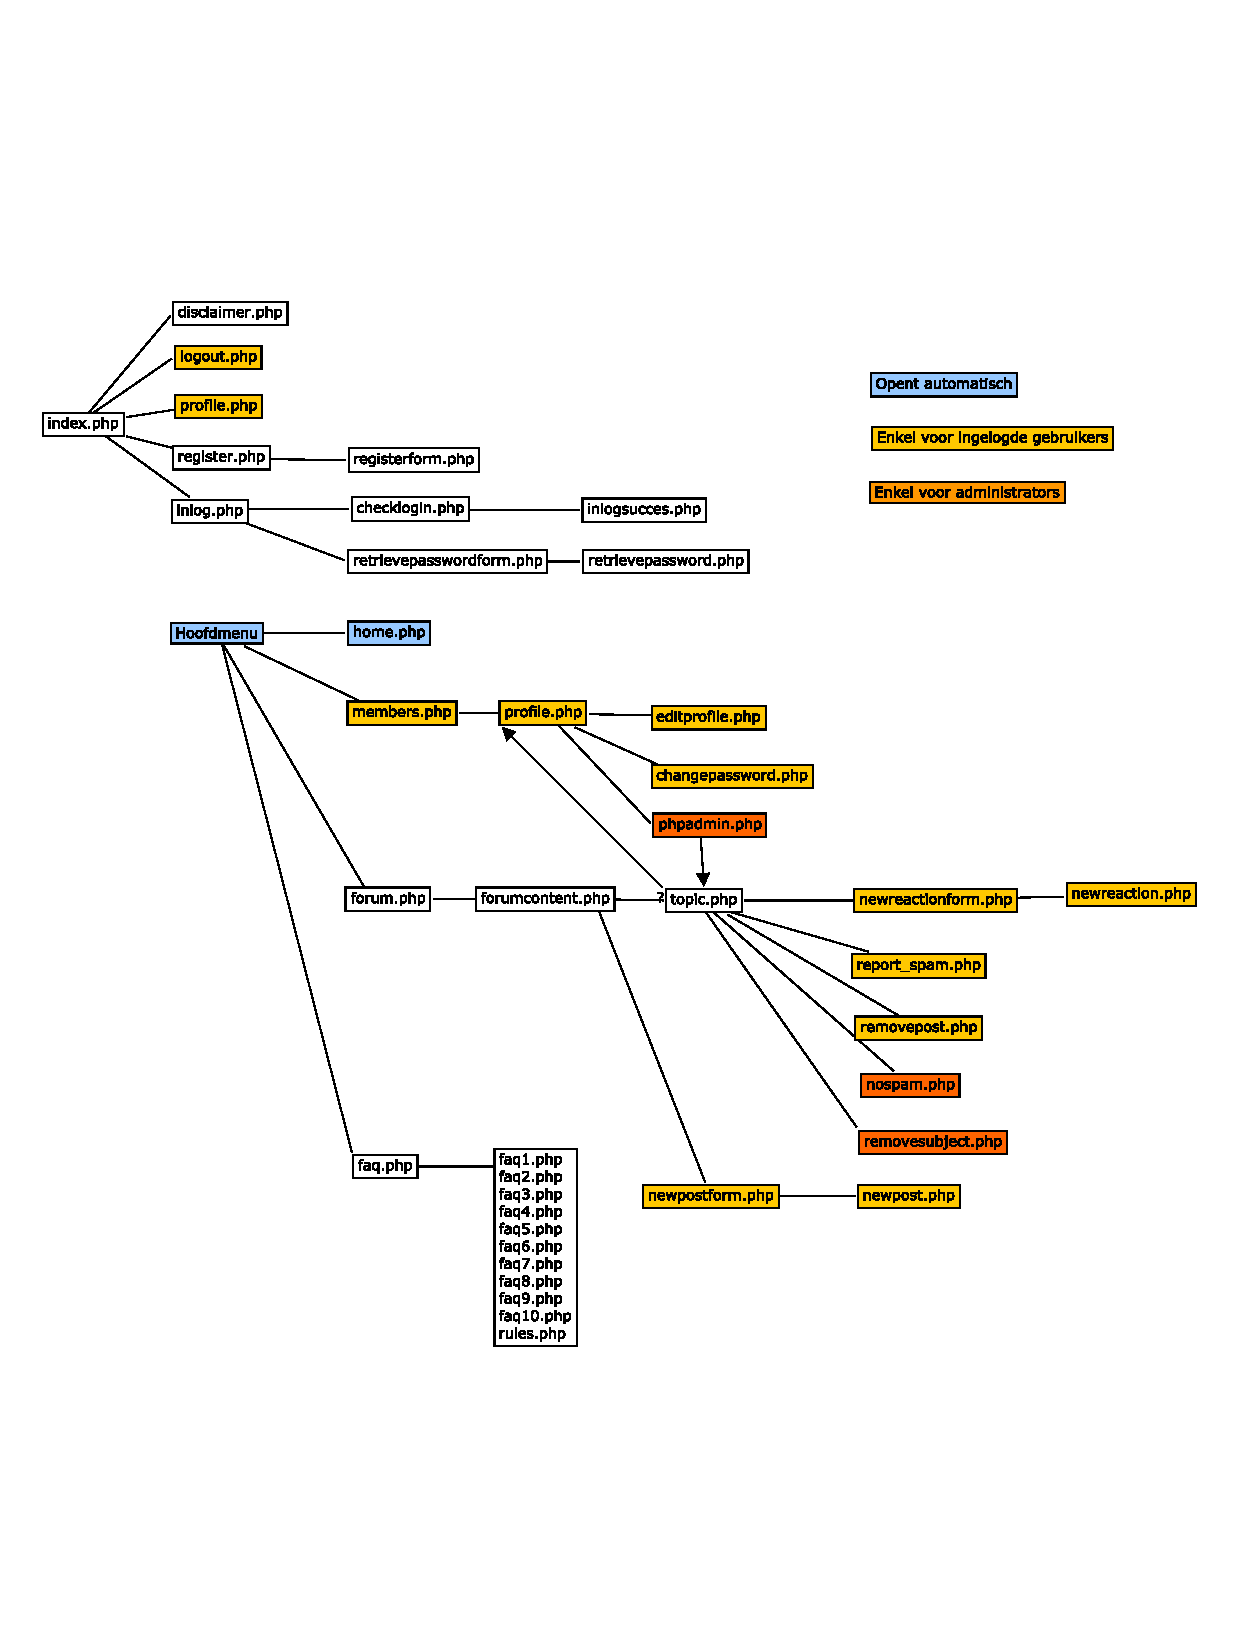
\includepdf[pages=-]{webstructuur.pdf} 
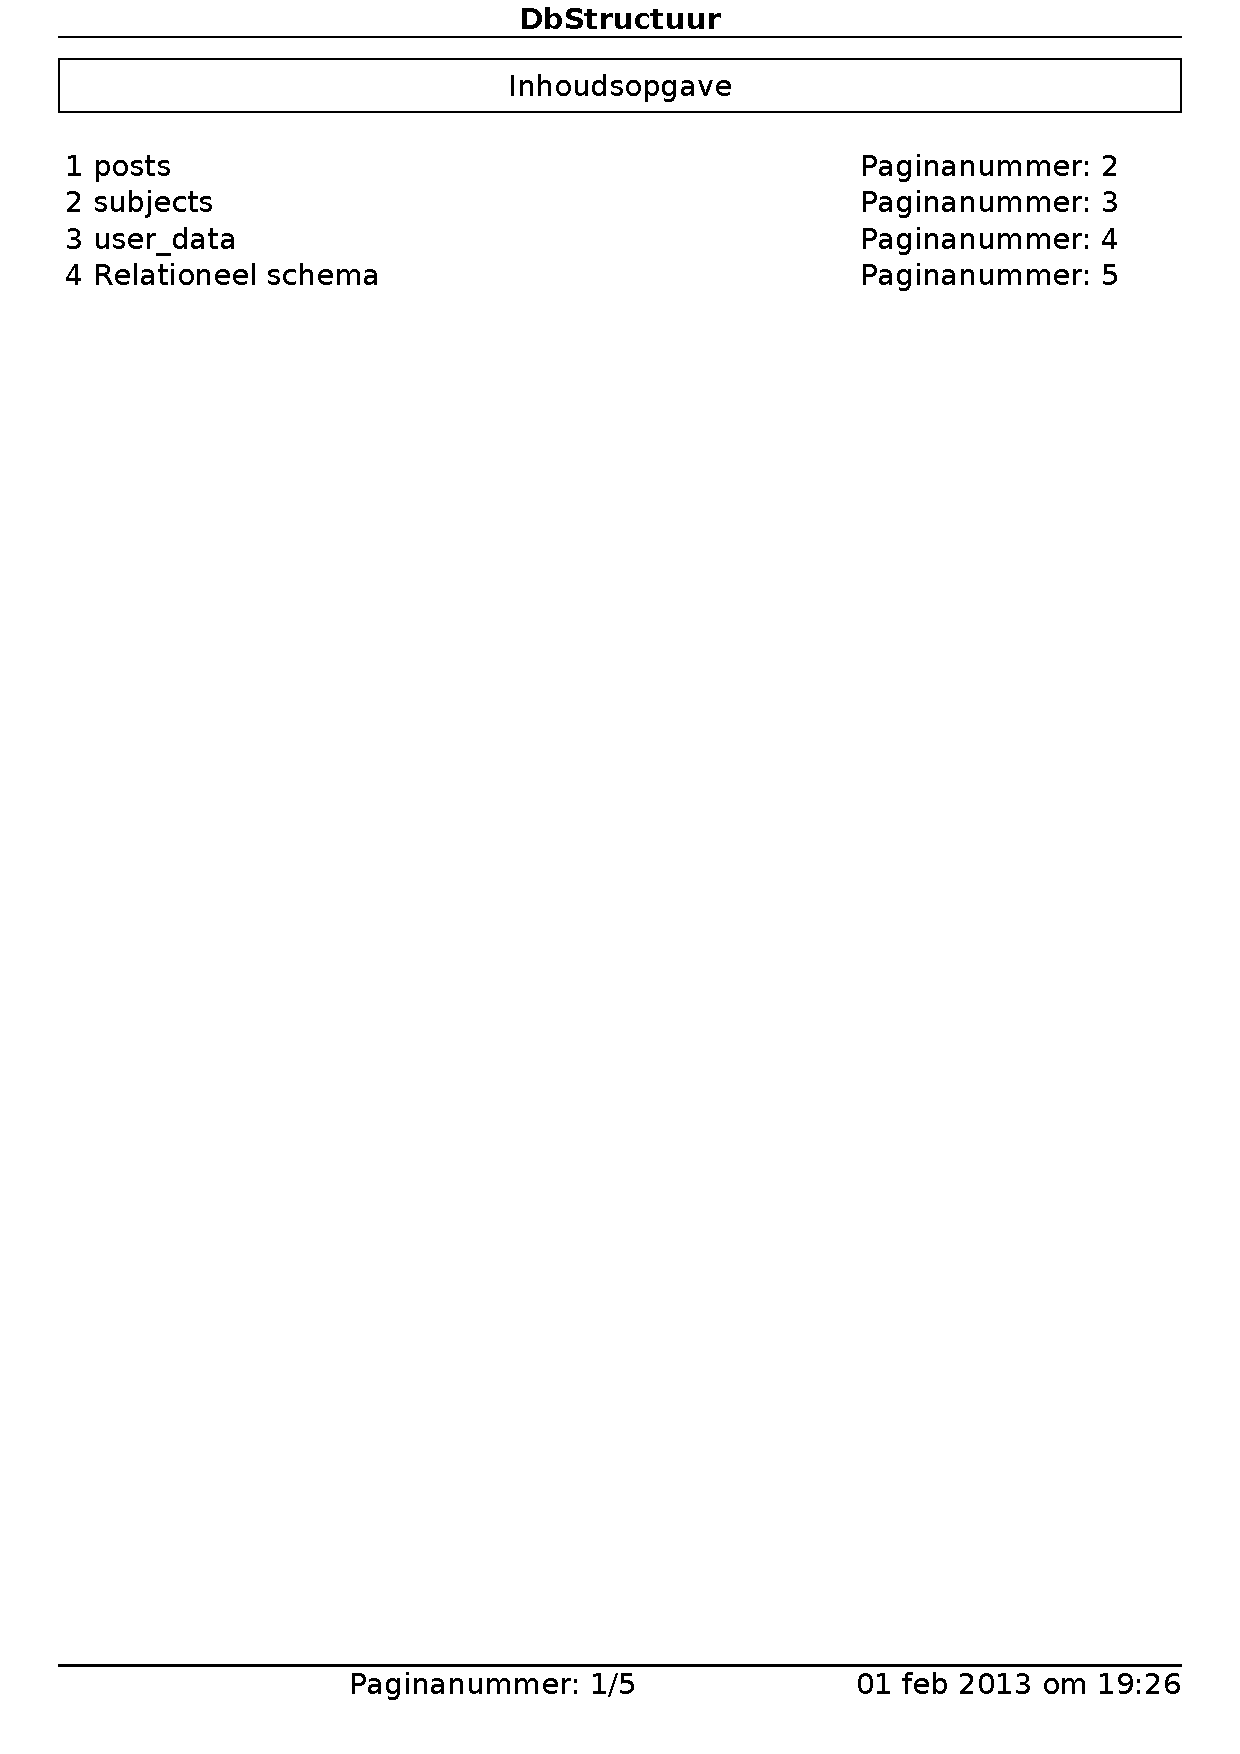
\includepdf[pages=-]{dbStructuur.pdf} 

\end{document}